

%%%%%%%%%%%%%%%%%%%%%%%%%%%%%%%%%%%%%%%%%%%%%%%%%%%%%%%%%%%%%%%%%%%%%%%%%%%%%%%%
\subsection{Architecture}

The footstep evaluation neural network architecture is shown in
\autoref{fig:diagram-contactnet-architecture} accomplishes a similar
task to ContactNet \cite{bratta_contactnet_2024}. It takes in terrain
and state information and ranks each of the possible footstep
positions. This network uses a multi-modal middle fusion
architecture. This architecture was chosen to effectively combine the
spatial features from the terrain data with the contextual features
from the robot state data, while still maintaining flexibility in
case re-training is needed \cite{feng2021deep}. The terrain data is
processed through a convolutional layer and fully connected layer,
while the robot state data is processed through fully connected
layers. The outputs of these two branches are then concatenated and
passed through an additional fully connected layer to produce the
final output, which consists of preference ratings for each potential
footstep position.

\begin{figure}
  \centering
  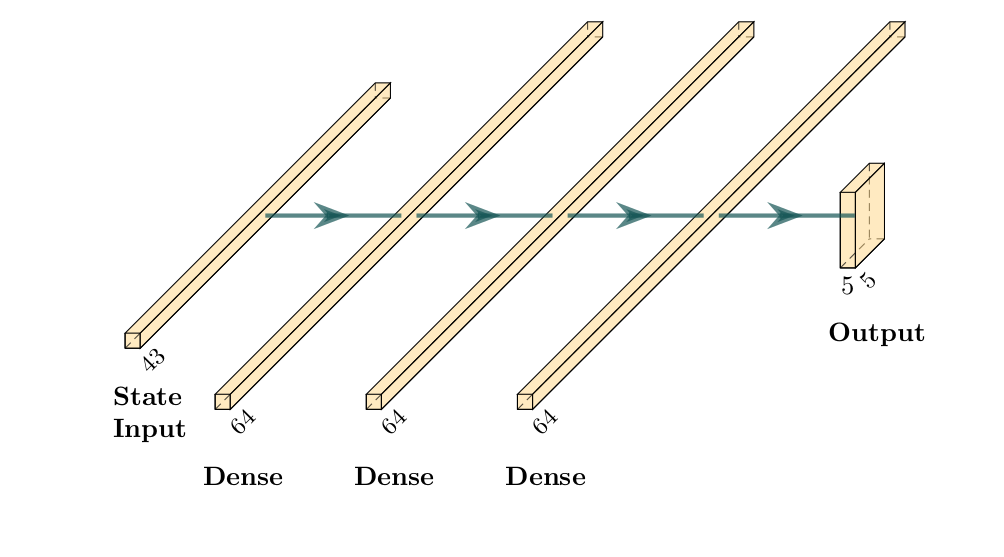
\includegraphics[width=0.5\linewidth]{images/diagrams/contact-network-architecture.png}
  \caption{Footstep evaluation neural network architecture.}
  \label{fig:diagram-contactnet-architecture}
\end{figure}

%%%%%%%%%%%%%%%%%%%%%%%%%%%%%%%%%%%%%%%%%%%%%%%%%%%%%%%%%%%%%%%%%%%%%%%%%%%%%%%%
\subsection{Training}
